%%-*- mode: LaTeX; mode: FlySpell; -*-

\section{Abstraction over events}
\label{sec:event}


\paolothree{
In Section~\ref{sec:prov-constraints} we recalled the definition of PROV ordering constraints C2-C5, given in the PROV-CONSTRAINT document, which must be satisfied by any valid PROV graph.
We now extend the notion of validity to events defined on  abstract graphs $G^{A}$.
}
\paolothree{ In general these are not the same events as $G^{C}$'s, because when $G^{A}$ is obtained using either e-grouping or a-grouping over some concrete base graph $G^{C}$, both entities and relationships may have changed.
Specifically, when $a_{new}$ is created through a-grouping, $G^{A}$'s events include 
 $start(a_{new})$, $end(a_{new})$, as well as 
$ev(\used(e, a_{new}))$, $ev(\wgby(a_{new}, e))$ for all $e$ that are generated by or used by $a_{new}$. 
For e-grouping, the new events are $ev(\wgby(e_{new}, a))$ and  $ev(\used(e_{new},a))$ for any $a$ that has generated (resp. used) $e_{new}$.
%
We are going to refer to the two sets of events in $G^{C}$ and $G^{A}$ as $\EVc$, $\EVa$, respectively.
}

\jwbthree{Note that} \jwbtwo{until this point we have been using single edges between nodes. 
Abstraction, however, can create single relations from more than one concrete relation.  PROV allows multiple edges between the same nodes to be distinguished using identifiers, and in this section we  introduce identifiers on relations to allow us to develop the abstract event preorder on the abstract graph that is consistent with the preorder on the concrete graph.}
\paolotwo{We use symbols such as $g_{41}$, as in Fig.~\ref{fig:e4-e5}, to indicate relationships like $\wgby(e_4, a_1)$. 
With slight abuse of notation, but in the interest of simplicity, in the following we are going to use $g_{41}$ to also denote $ev(\wgby(e_4, a_1))$ when it is clear from the context that we refer to the event rather than to the relationship itself.
}

\begin{figure*}
	\centering
	%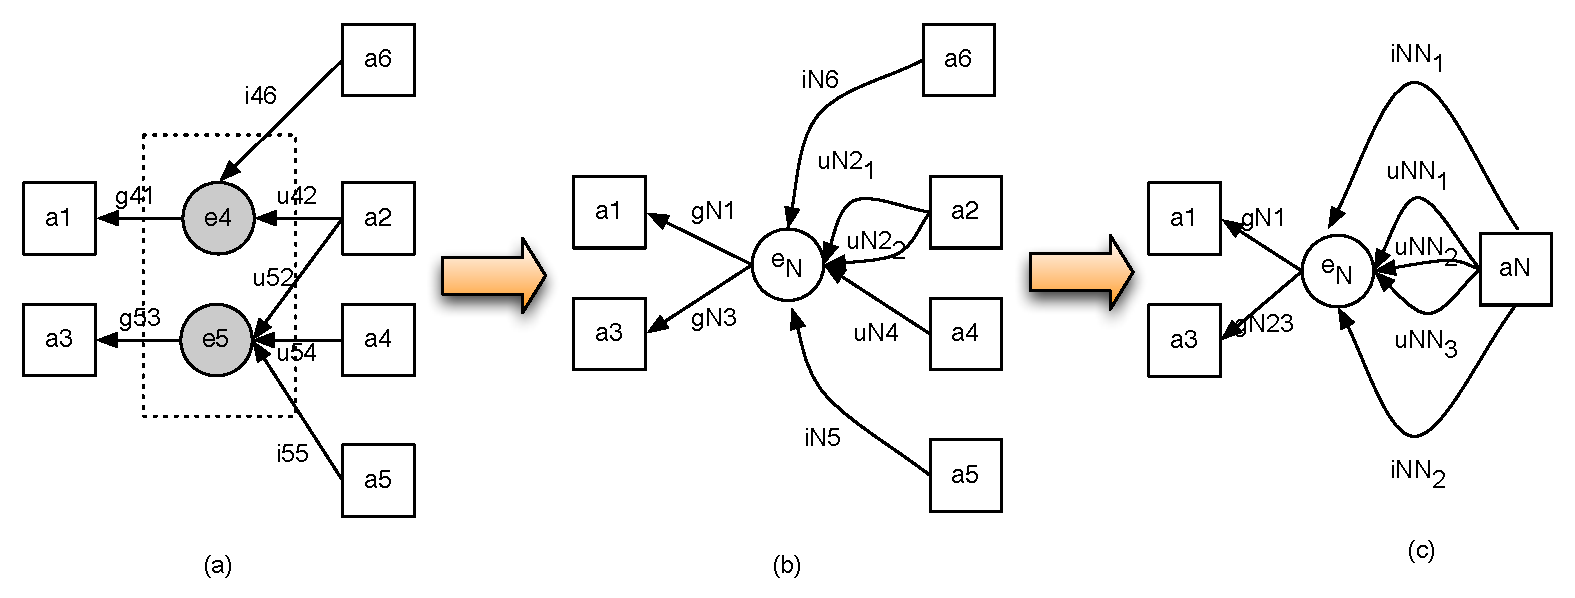
\includegraphics[scale=.5]{figures/e4-e5.pdf} 
	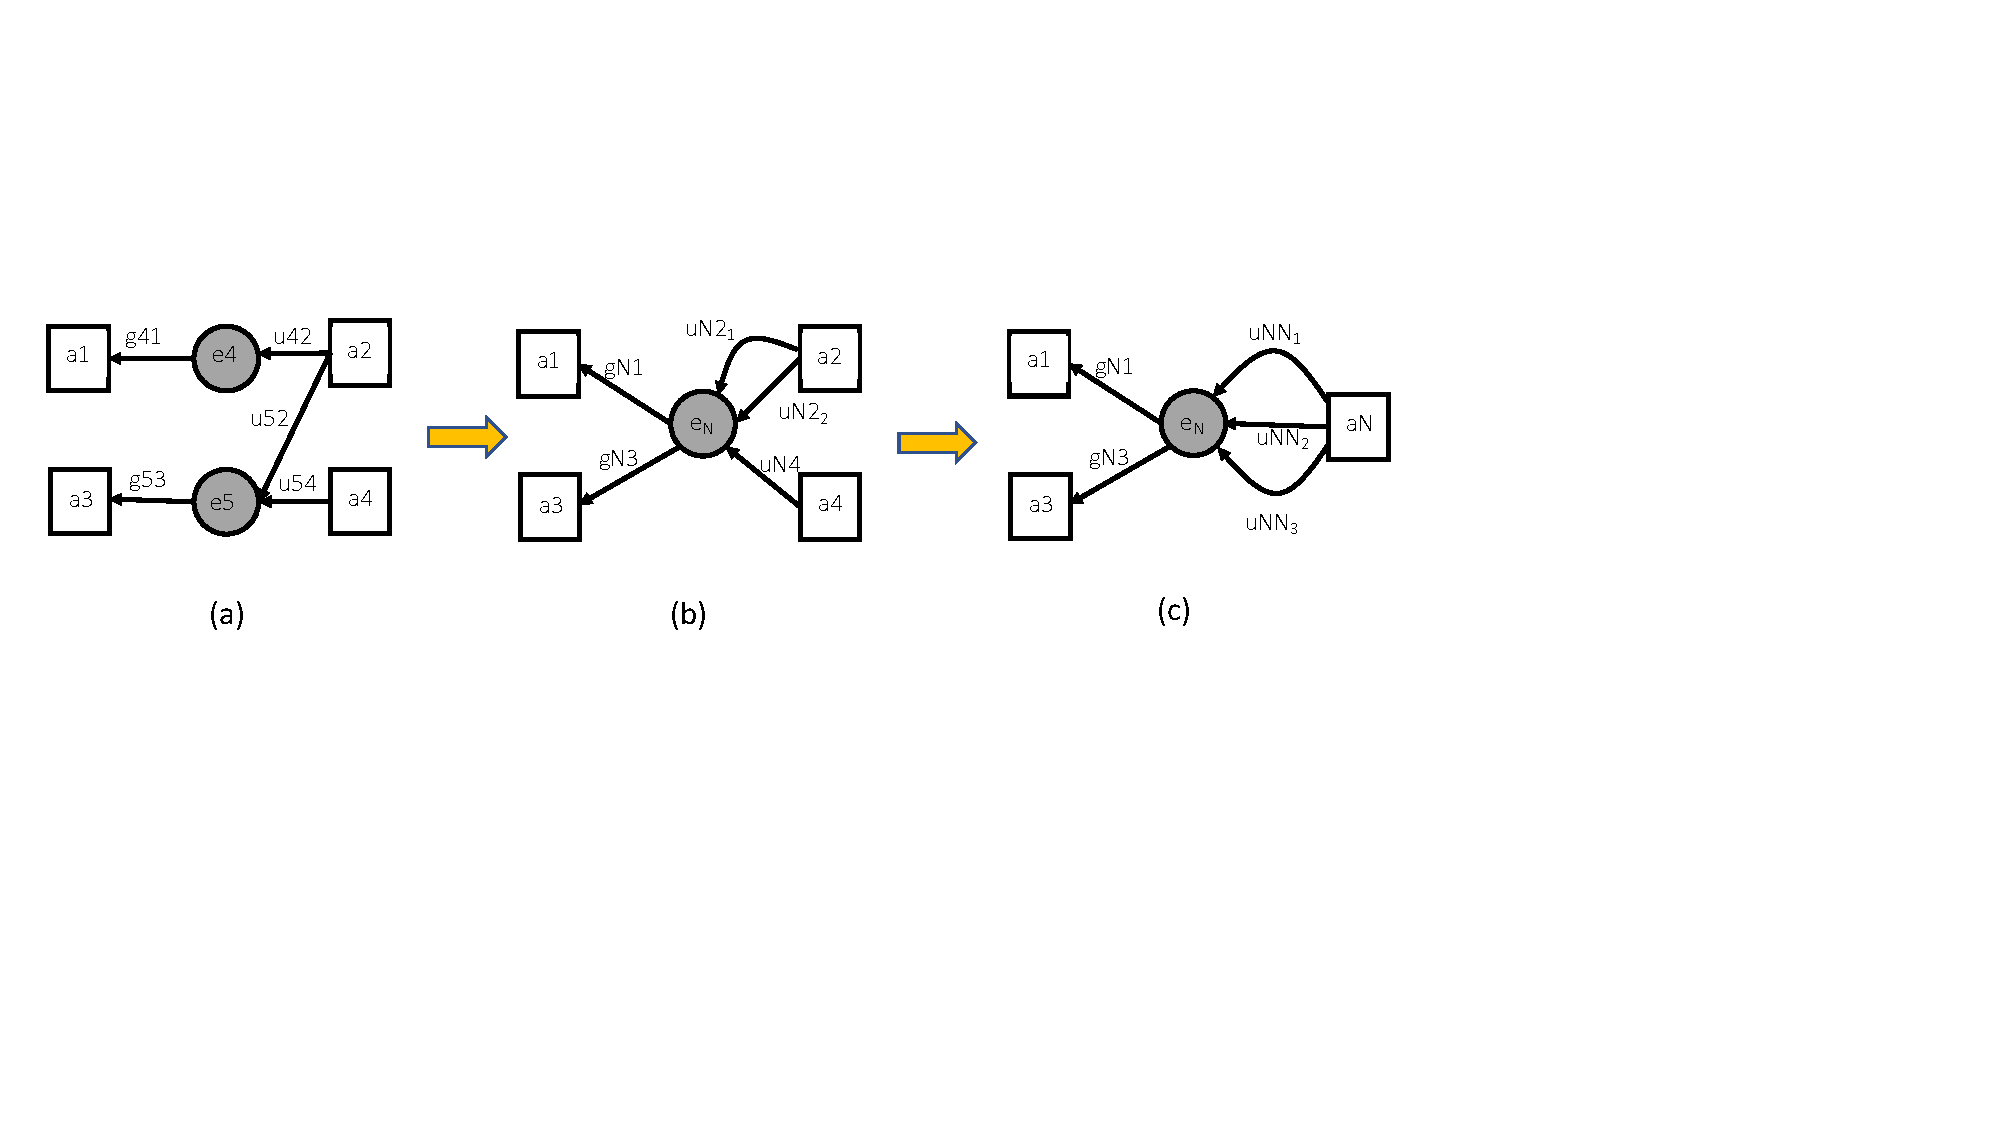
\includegraphics[scale=.5]{cropped-reworked-e4-e5.pdf} 
	\caption{Abstraction over a document content, and associated abstracted events} \label{fig:e4-e5}
\end{figure*}



\paolotwo{To fix ideas, consider $G^{C}$ in Fig.~\ref{fig:e4-e5}(a), where two sections of a document are independently generated by two editing activities, and then they are independently used by \jwbthree{two} more activities. Note that this is a slight extension of the abstract pattern of Fig.~\ref{fig:e2-a4}, where the document sections are $e_4$, $e_5$.
%
The e-grouping set $V_{gr} = \{ e_4, e_5\}$ represents the whole document. 
}

\paolothree{
	The argument in this section is focused on e-grouping and generation-usage constraints, and omits similar logic which applies to a-grouping and to other temporal constraints.
}
\paolotwo{	Let $G^{A}$ be the result of (non-strict) e-grouping, as depicted in Fig.~\ref{fig:e4-e5}(b), where the abstract generation and usage events are given new names, namely $g_{Ni}$ as a shorthand for $\wgby(e_N,a_i)$, and $u_{Ni_j}$ for each usage $j$ of the form $\used(a_i, e_N)$. \jwbthree{ The form $u_{Ni_j}$ is only needed when multiple $used$ relationships link the same two nodes.}
\sloppy Thus, $\EVc = \{ g_{41}, g_{53}, u_{42}, u_{52}, u_{54} \}$ and $\EVa = \{ g_{N1}, g_{N3}, u_{N2_1}, u_{N2_2}, u_{N4} \}$.
%
If $G^{C}$ is valid, by constraint C3 the following must hold:
\begin{align}
\label{eq:c3-G}
g_{41} \preorder u_{42}, \quad g_{53} \preorder u_{52}, \quad g_{53} \preorder u_{54} 
\end{align}
where $\preorder$ is the preorder relationship introduced in Section~\ref{sec:prov-events}.
}
\paolothree{
	Importantly, note however that $g_{41} \preorder u_{54}$ does not hold.}
\paolotwo{Similarly, for $G^{A}$ to be valid we must have:
\begin{align}
g_{N1} \preorder u_{N2_1}, \quad g_{N1} \preorder u_{N2_2}, \quad g_{N1} \preorder u_{N4}  \label{eq:c3-global1} \\  
g_{N3} \preorder u_{N2_1}, \quad g_{N3} \preorder u_{N2_2}, \quad g_{N3} \preorder u_{N4} \label{eq:c3-global2} 
\end{align}}

\paolotwo{To understand multiple generation and usage events associated with the same entity, recall that PROV-DM~\citep{w3c-prov-dm} defines those events as follows:
%\begin{description}
\begin{itemize}
	\item\textbf{Generation} \textit{is the completion of production of a new entity by an activity} (Section 5.1.3 of~\citep{w3c-prov-dm})
	\item\textbf{Usage} \textit{is the beginning of utilizing an entity by an activity} (Section 5.1.4 of~\citep{w3c-prov-dm})
%	\item\textbf{Invalidation} \textit{is the start of the destruction, cessation, or expiry of an existing entity by an activity. The entity is no longer available for use (or further invalidation) after invalidation. Any generation or usage of an entity precedes its invalidation.} (Sec. 5.1.8)
\end{itemize}
}

\paolotwo{Thus, $e_{N}$ is generated when both generation events $g_{N1}, g_{N3}$ have occurred (by Constraint \jwbthree{C2 from} PROV-CONSTRAINTS, this implies that these abstract events must be simultaneous), and it starts being used when the ``earliest'' of the usage events takes place, keeping in mind that no ordering relationships amongst the usage events is necessarily defined.
}

\paolothree{
	We aim to establish a formal relationship between concrete and abstract events, and between temporal constraints amongst those events. 
Specifically, we will see that some constraints over events in $\EVc$ map directly to constraints in $\EVa$, but also that, to be valid, $G^A$ may require additional constraints that are not in $G^C$.
Thus, intuitively, we aim to show that validity of $G^A$ follows from validity of $G^C$, but only in part.
}

\subsection{Constraint C3 (generation precedes usage)}

\paolothree{
	For simplicity, consider initially the single temporal constraint C3 \jwbthree{(generation precedes usage)}, i.e., assume that the preorder on $\EVc$ satisfies C3.
We observe that Def.~\ref{def:var-in-out} (pg~\pageref{def:var-in-out}) effectively defines a mapping between relationships (graph arcs) in $G^C$ that cross the boundaries of a ``convex'' subgraph $V^*$ of $G^C$ obtained by closure $\pclos()$ and expansion ($\extend()$, for type consistency), and the new arcs in $G^A$.
Specifically, given $V^*$, Def.~\ref{def:var-in-out}  provides the basis for the $\repl()$ operator, by mapping:
\begin{align}
\text{arcs: }  v \xleftarrow{ty} v' \in \vartheta_{out}(V^*)  \text{ to arcs  } v \xleftarrow{ty}  v_{new}; \\
\text{arcs: } v' \xleftarrow{ty} v \in \vartheta_{in}(V^*) \text{ to arcs  }v_{new} \xleftarrow{ty} v;\\
\text{arcs: in } \vartheta_{int}(V^*) \text{ to themselves}.
\end{align}
In turn, this defines a mapping between concrete and abstract events corresponding to the arcs ($\wgby$ and $\used$). 
We denote such mapping by: 	 
\begin{align}
\psi: \EVc \rightarrow \EVa
\end{align}
For example, for the events in Fig.~\ref{fig:e4-e5}(a) and (b) the mappings are: $\psi(g_{41}) = g_{N1}$, $\psi(u_{42}) = u_{N2_1}$, $\psi(u_{54}) = u_{N4}$, etc.
By the nature of $\repl()$, the only interesting constraints covered by $\psi()$ relate to events that occur on the boundary of $V^*$.
}

\paolothree{
	In this example, note that $g_{41} \preorder u_{42}$ holds in $G^C$, and $\psi(g_{41}) = g_{N1} \preorder u_{N2_1} = \psi(u_{42})$ holds in $G^A$, that is, $\psi()$ preserves the order in $G^C$.
But for instance, for $G^A$ to be valid, $g_{N1} \preorder u_{N4}$ must also hold, which however does not follow from a corresponding constraint in $G^C$, in fact $g_{41}$ and $u_{54}$ are unrelated.
Thus, intuitively we expect to be able to ``explain'' only some of the constraints in $G^A$ in terms of constraints on $G^C$.
}

\paolothree{
	To formalise this idea, and observing that $\psi()$ is injective and total, thus invertible, we define the \textit{support} of a constraint in $G^A$ as follows.
}

\paolothree{
	\begin{definition}[Support of constraint C3 in $G^A$]  \label{def:support}
	Let $g' = (a_1 \leftarrow e_N), u' = (e_N \leftarrow a_2) \in \EVa$ be two generation and usage events, respectively, associated with abstract entity node $e_N$.
    For $G^A$ to be valid relative to C3, $g' \preorder u'$	must hold. 
    The support of $g' \preorder u'$ in $G^C$ is defined as the constraint $\psi^{-1}(g') \preorder \psi^{-1}(a').$    
\end{definition}
}

\paolothree{
	\begin{proposition}[Condition for support]  \label{prop:support}
	Let $g' = (a_1 \leftarrow e_N), u' = (e_N \leftarrow a_2) \in \EVa$, $g' \preorder u'$ be a constraint as in Def.~\ref{def:support}, and let 	
	$\psi^{-1}(g')  = (a'_1 \leftarrow e_y), \psi^{-1}(a') =  (e_x \leftarrow a'_2) \in \EVc$.
	The support of $g' \preorder a'$ is defined in $G^C$ only if there a path from $e_x$ to $e_y$ in $V^*$.	
\end{proposition}
}

\begin{figure*}
	\centering
	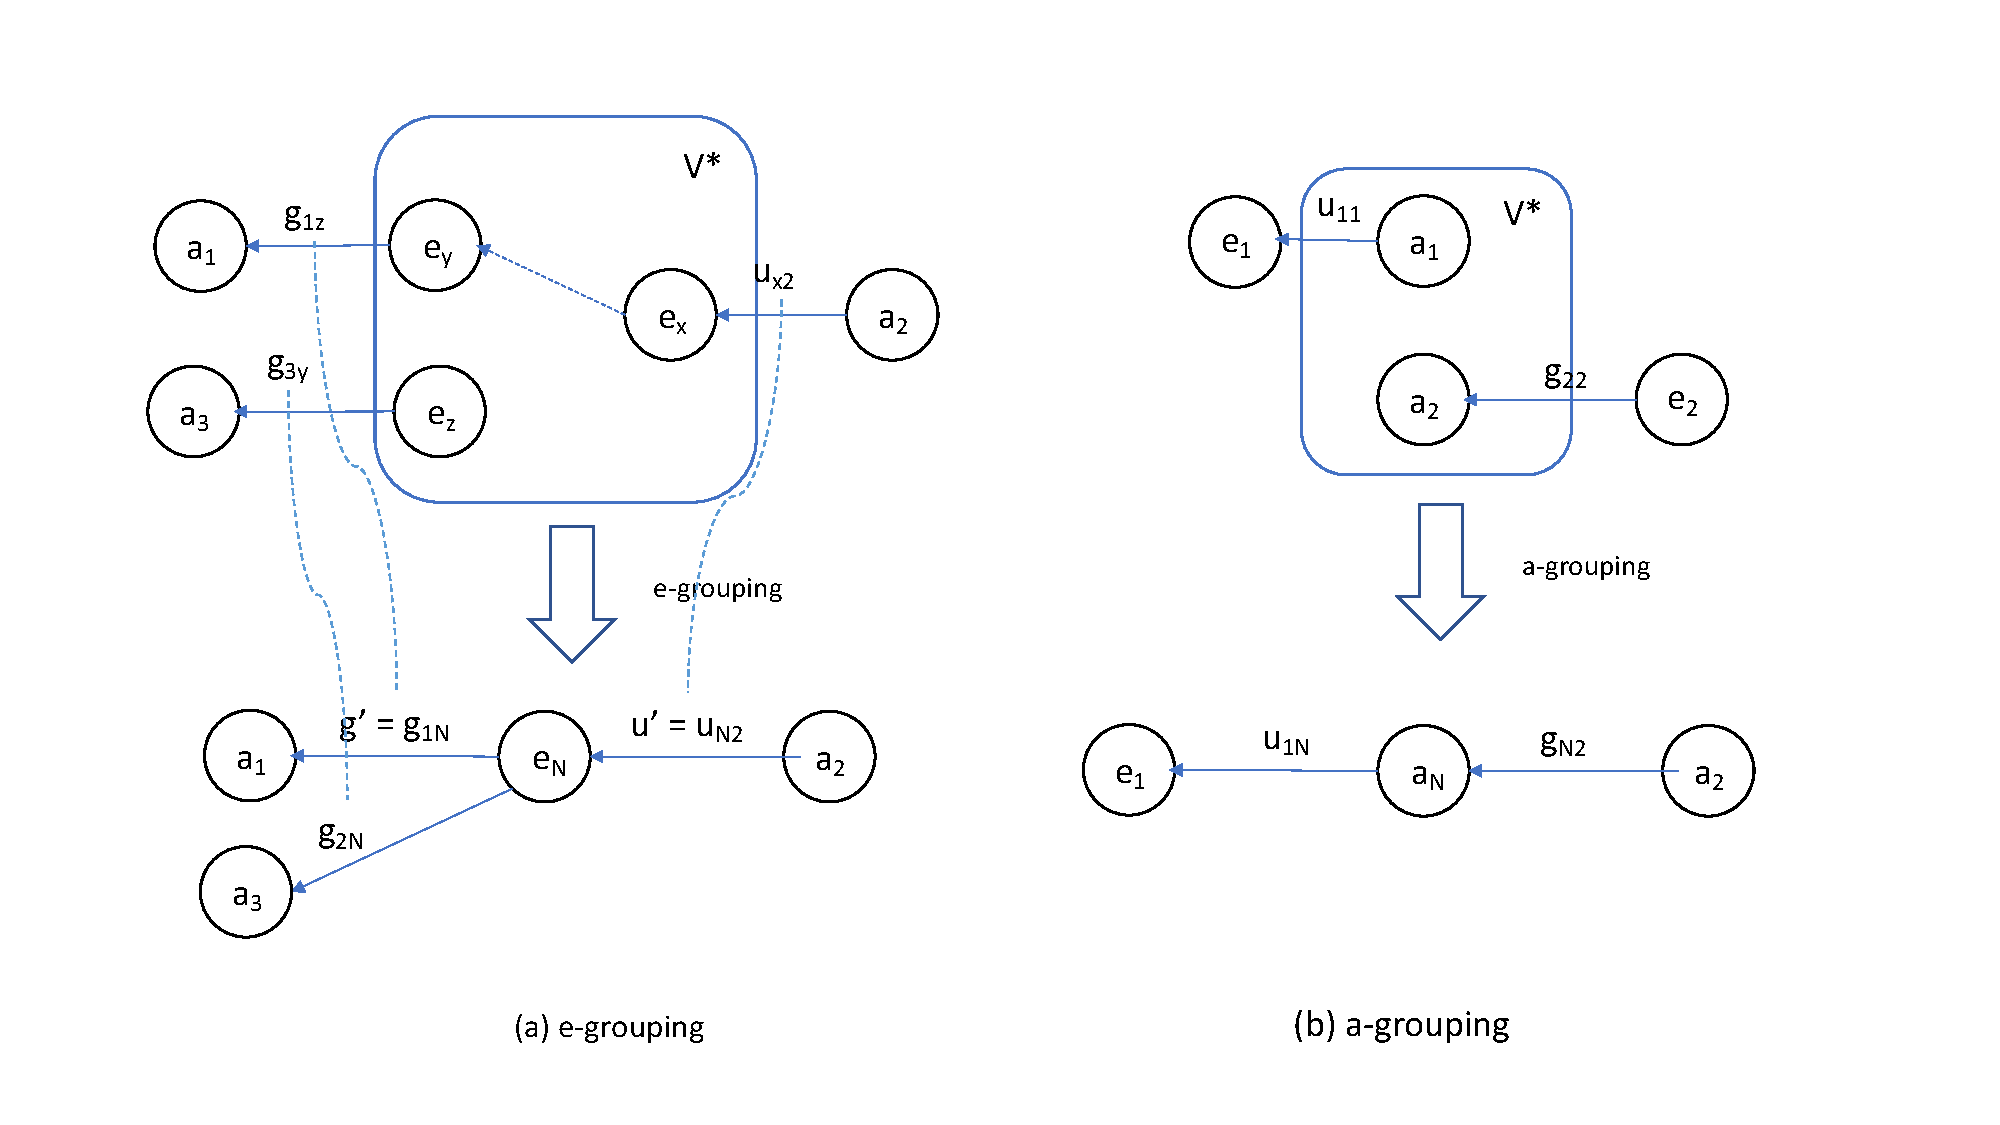
\includegraphics[scale=.4]{figures/example-abstract-events.pdf} 
	\caption{Paths within $V^*$ determine temporal constraints in the abstract graph.} \label{fig:events-e-grouping}
\end{figure*}



\begin{pf}
\paolothree{
Firstly, observe that $\psi^{-1}(g') \in \vartheta_{out}(V^*) $ and $\psi^{-1}(u') \in \vartheta_{in}(V^*) $. 
These both follow directly from our definition of $\psi()$.
Also, $a_1 = a'_1$ and  $a_2 = a'_2$.
Thus, the situation is as depicted in Fig.~\ref{fig:events-e-grouping}(a), showing the generation and usage events on the boundaries of $V^*$.
If there is a path from $e_x$ to $e_y$, then this must form a chain of generation-usage relationships, and by transitivity of the preorder, this entails $g_{1y} = (a_1 \leftarrow e_y ) \preorder (e_x \leftarrow a_2) = u_{x2}$, which is the support of $g' \preorder a'$.
}

\paolothree{
On the other hand, consider the constraint $(a_3 \leftarrow e_N) \preorder (e_N \leftarrow a_2)$.
Its support is $(a_3 \leftarrow e_z ) \preorder (e_x \leftarrow a_2)$, however if there is no path from $e_x$ to $e_z$, we cannot entail this constraint through transitivity, \jwbthree{and} in fact there is no such constraint in $G^C$.
}
\end{pf}

\paolothree{
The example in Fig.~\ref{fig:e4-e5} shows a similar scenario, as noted above.
%
Thus, the dependencies within $V^*$ determine which additional constraints must hold in the abstract graph, that \jwbthree{do not} hold in the concrete graph.
We can provide a simple interpretation of this situation, by considering the set of all possible total orderings amongst events in $\EVc$, or \textit{unfoldings} of $G^C$, that are consistent with the temporal constraints in $G^C$.
It should be clear that adding constraints reduces the number of unfoldings. 
}
\paolothree{
Thus, we have shown that ensuring validity of $G^A$ may require constraints that correspond to \textit{new} constraints that did not need to hold in $G^C$. 
We could say that $G^A$ represents only a fragment of the unfoldings of $G^C$. In the example, these are only the unfoldings where $g_{41} \preorder u_{54}$ is true.
}

\subsection{Constraints C2, C4, C5}
\paolothree{
	%
	Regarding C2 (generation-generation ordering), we have again that new constraints on abstract events need to hold  in $G^A$, even when those are mapped from concrete events that are unrelated.
	For example, consider again Fig.~\ref{fig:e4-e5} where $g_{41}$ and $g_{53}$ are unrelated, yet in $G^A$, the corresponding abstract events must be simultaneous, because both are associated wth the generation of $e_N$:$\psi(g_{41}) \preorder \psi(g_{53})$ and $\psi(g_{53}) \preorder \psi(g_{41})$.
	Generalising from the example, it is straighforward to see that for any pair of generation events $g, g' \in \vartheta_{out}(V^*) $ in $G^A$ the following must hold:
	\[    \psi(g) \preorder \psi(g'), \quad \psi(g') \preorder \psi(g)\]
}	



\paolothree{
Regarding C4 and C5, intuitively these constraints state that any entity generation and usage events must ``lie within''  the interval defined by the start and end events for the relevant activities. 
%
	Consider Fig.~\ref{fig:events-e-grouping}(b), with constraints:
	\begin{align}
	\start(a_N) \preorder u_{1N} \preorder \ed(a_N) \\
	\start(a_N) \preorder g_{N2} \preorder \ed(a_N)
	\end{align}
	%	
	We would like to define $\start(a_{N})$, $\ed(a_{N})$ in terms of corresponding concrete events, i.e., $\start(a_{1})$, $\ed(a_{1})$  and $\start(a_{2})$, $\ed(a_{2})$, so that we can determine the relationship between the two.
	Our construction of $\psi()$ does not help here, however, because $\psi()$ is defined on constraints (usage, generation) that are associated with edges in the abstract graph, whereas these activity constraints are associated to (activity) nodes.
	%
	The problem is that, to the best of our knowledge, PROV-CONSTRAINTS does not offer an intution to define such mappings. 
	Unlike for ``composite'' entities, where usage and generation can be defined as we have done at the start of this section, there seems to be no corresponding notion of ``compound activity'' where the start and end events of the composite are defined in terms of those of its components.\footnote{There is a notion of one activity starting or ending other activities, but that does not seem to help with the mapping we are seeking.}
	Thus, we regard further investigations involving constraints C4, C5 as out of scope, and as an open problem.
}	
	 
%\paolothree{	It is hopefully easy to see, however, that the same logic that emerges from  Fig.~\ref{fig:events-e-grouping}(a) and has been used in Prop.~\ref{prop:support} applies when are considered. 
%	%
%%	We can see in Fig.~\ref{fig:events-e-grouping} that, for example, $\start(a_2) \preorder u_{N2} \preorder \ed(a_2) must hold in $G^A$, but these two constraints have no support in $G^C$: 
%%	$\psi^{-1}( \start(a_2) \preorder u_{N2} ) \preorder \psi^{-1}(a').$  
%	%	$\start(a_1) \preorder g_{12} \preorder \ed(a_1)$, must hold, but $g_{12}$ is unrelated to start and end events in $a_2$.
%%
%}
% 
